\documentclass[aspectratio=169, 10pt]{beamer}

% Theme configuration
\usetheme{Madrid}
\usecolortheme{whale}

\usepackage{tikz}
\usetikzlibrary{shapes.geometric, arrows.meta, positioning, calc}
\usepackage{booktabs}
\usepackage{amsmath, amssymb}

% Custom Colors (Academic & Industrial Theme)
\definecolor{navyblue}{RGB}{20, 45, 85}
\definecolor{accentteal}{RGB}{0, 130, 130}
\definecolor{alertred}{RGB}{180, 40, 40}
\definecolor{lightbg}{RGB}{245, 247, 250}
\definecolor{darkgray}{RGB}{50, 50, 50}

\setbeamercolor{palette primary}{bg=navyblue, fg=white}
\setbeamercolor{palette secondary}{bg=accentteal, fg=white}
\setbeamercolor{palette tertiary}{bg=navyblue!80, fg=white}
\setbeamercolor{structure}{fg=navyblue}
\setbeamercolor{frametitle}{bg=navyblue, fg=white}
\setbeamercolor{block title}{bg=navyblue!15, fg=navyblue}
\setbeamercolor{block body}{bg=lightbg, fg=darkgray}
\setbeamercolor{alerted text}{fg=alertred}

% Metadata
\title[Phase 3: Neural Instrumentation]{Phase 3: Neural Network Instrumentation}
\subtitle{Unified ModelInspector Framework for Mechanistic Interpretability}
\author[Brian A. Hadian]{Brian A. Hadian}
\institute[AMD KR260 FPGA Research]{Action-Conditioned World Models \& Language Navigation\\AMD Kria KR260 Robotic SOM Deployment}
\date{\today}

\begin{document}

% -----------------------------------------------------------------------------
% Slide 1: Title Slide
% -----------------------------------------------------------------------------
\begin{frame}
  \titlepage
\end{frame}

% -----------------------------------------------------------------------------
% Slide 2: Making Computation Observable Without Interference
% -----------------------------------------------------------------------------
\begin{frame}{1. Making Internal Computation Fully Observable}
  \textbf{Core Insight:} \textit{Neural instrumentation must render intermediate states observable without altering model execution semantics.}

  \vspace{0.3cm}
  \begin{columns}[T]
    \begin{column}{0.55\textwidth}
      \begin{block}{The Non-Interference Mandate}
        \small
        \begin{itemize}
          \item In mechanistic discovery, any side effect from monitoring (e.g., in-place tensor modification or memory leakage) invalidates causal conclusions.
          \item The \textbf{\texttt{ModelInspector}} decouples observation from forward execution by using detached tensor cloning.
        \end{itemize}
      \end{block}
      
      \vspace{0.2cm}
      \begin{alertblock}{Rigorous Acceptance Criterion}
        \small
        Clean unhooked output vs. hooked output maximum absolute difference must satisfy:
        $$\|\mathbf{y}_{\text{hooked}} - \mathbf{y}_{\text{clean}}\|_\infty = 0.00 \times 10^0$$
      \end{alertblock}
    \end{column}

    \begin{column}{0.42\textwidth}
      \small
      \begin{center}
        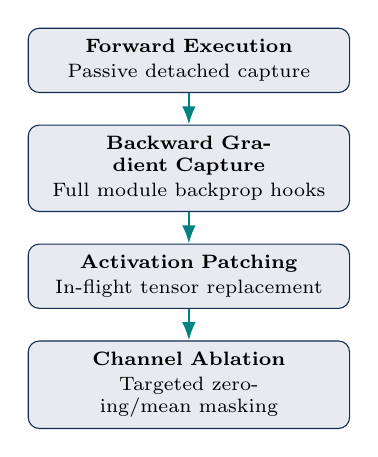
\begin{tikzpicture}[node distance=0.4cm and 0.5cm, auto, >=Latex]
          \tikzstyle{ibox} = [rectangle, rounded corners, draw=navyblue, fill=navyblue!10, inner sep=4pt, text width=3.8cm, align=center, font=\scriptsize]
          \node[ibox] (i1) {\textbf{Forward Execution}\\[1pt]Passive detached capture};
          \node[ibox, below=of i1] (i2) {\textbf{Backward Gradient Capture}\\[1pt]Full module backprop hooks};
          \node[ibox, below=of i2] (i3) {\textbf{Activation Patching}\\[1pt]In-flight tensor replacement};
          \node[ibox, below=of i3] (i4) {\textbf{Channel Ablation}\\[1pt]Targeted zeroing/mean masking};
          
          \draw[->, thick, accentteal] (i1) -- (i2);
          \draw[->, thick, accentteal] (i2) -- (i3);
          \draw[->, thick, accentteal] (i3) -- (i4);
        \end{tikzpicture}
      \end{center}
    \end{column}
  \end{columns}
\end{frame}

% -----------------------------------------------------------------------------
% Slide 3: Ten Mandatory Representations Captured Across Three Models
% -----------------------------------------------------------------------------
\begin{frame}{2. Ten Mandatory Representations Cataloged}
  \textbf{Core Insight:} \textit{All 10 required representations are bound to specific PyTorch submodules across all three architectures.}

  \vspace{0.2cm}
  \begin{center}
    \footnotesize
    \begin{tabular}{clllc}
      \toprule
      \textbf{\#} & \textbf{Representation Concept} & \textbf{Baseline Policy} & \textbf{LeWorldModel (LeWM)} & \textbf{H-JEPA} \\
      \midrule
      1 & Raw Image Embedding & \texttt{encoder.fc} ($z$) & \texttt{encoder[10]} ($s_t$) & \texttt{encoder[10]} ($s_t$) \\
      2 & Goal Embedding & \texttt{goal\_vec} (dim 4) & \texttt{target\_pose} (dim 3) & \texttt{target\_pose} (dim 3) \\
      3 & Current World-State & \texttt{encoder.fc} & \texttt{encoder[10]} & \texttt{encoder[10]} \\
      4 & Action Embedding & \texttt{actions} (dim 3) & \texttt{actions} to \texttt{pred\_fc1} & \texttt{actions} to \texttt{macro\_fc1} \\
      5 & Predicted Future Rep & --- & $s_t + \Delta s$ & $S_k + \Delta S$ / $s_t + \Delta s$ \\
      6 & Prediction Residual & --- & \texttt{pred\_delta} ($\Delta s$) & \texttt{macro\_predictor.delta} \\
      7 & Macro-Level Latent & --- & --- & $\hat{S}_{k+1}$ ($K=5$) \\
      8 & Micro-Level Latent & --- & --- & $\hat{s}_{t+1}$ ($K=1$) \\
      9 & Policy Output & \texttt{action\_head} & Latent MPC Selector & \texttt{micro\_predictor.action} \\
      10 & Controller Output & \texttt{collision\_head} & \texttt{col\_fc} logit & \texttt{macro\_predictor.col} \\
      \bottomrule
    \end{tabular}
  \end{center}

  \vspace{0.1cm}
  \begin{block}{Architectural Decoupling}
    \scriptsize
    For H-JEPA, macro ($K=5$) and micro ($K=1$) tiers are tapped independently; for LeWM, the encoder and predictor pathways are separated into distinct hook namespaces.
  \end{block}
\end{frame}

% -----------------------------------------------------------------------------
% Slide 4: Active Interventions: Activation Patching & Channel Ablations
% -----------------------------------------------------------------------------
\begin{frame}{3. Active Interventions: Patching \& Channel Ablations}
  \textbf{Core Insight:} \textit{In-flight tensor replacement enables controlled causal attribution tests without model fine-tuning.}

  \vspace{0.3cm}
  \begin{columns}[T]
    \begin{column}{0.5\textwidth}
      \begin{block}{Activation Patching Context}
        \small
        \begin{itemize}
          \item Temporarily replaces a layer's output tensor $\mathbf{h}_l$ with a counterfactual activation $\mathbf{h}_l^*$.
          \item Measures the direct downstream output shift $\Delta \mathbf{y} = \|\mathbf{y}(\mathbf{h}_l^*) - \mathbf{y}(\mathbf{h}_l)\|$.
          \item Verified on Baseline latent $z$: output shifted by \textbf{$0.5157$}, proving active causal intervention.
        \end{itemize}
      \end{block}
    \end{column}

    \begin{column}{0.48\textwidth}
      \begin{alertblock}{Feature Channel Ablation Context}
        \small
        \begin{itemize}
          \item Zeroes out or mean-imputes individual latent channels (e.g., channels $0, 1, 2$).
          \item Verified on Baseline latent $z$: 3-channel ablation shifted actuator output by \textbf{$0.1402$}.
          \item Essential for isolating which individual neurons encode obstacle clearance in Phase 5.
        \end{itemize}
      \end{alertblock}
    \end{column}
  \end{columns}
\end{frame}

% -----------------------------------------------------------------------------
% Slide 5: Configurable Three-Tier Trace Serialization
% -----------------------------------------------------------------------------
\begin{frame}{4. Configurable Three-Tier Trace Serialization}
  \textbf{Core Insight:} \textit{Segregating full diagnostic dumps, selected latents, and running moments prevents memory bottlenecks.}

  \vspace{0.3cm}
  \begin{table}[h]
    \centering
    \small
    \begin{tabular}{llcl}
      \toprule
      \textbf{Logging Tier} & \textbf{Format} & \textbf{Storage Footprint} & \textbf{Intended Scientific Purpose} \\
      \midrule
      \textbf{Diagnostic Mode} & Compressed \texttt{.npz} & $\approx 435\,\text{KB}$ / 10 steps & Single-episode deep layer audits \& debugging \\
      \textbf{Selected Mode} & Compressed \texttt{.npz} & $\approx 1.2\,\text{KB}$ / 10 steps & Training Sparse Autoencoders (SAEs) in Phase 4 \\
      \textbf{Statistical Mode} & JSON Summary & $\approx 2.5\,\text{KB}$ total & Large-scale evaluation moments (mean, std, sparsity) \\
      \bottomrule
    \end{tabular}
  \end{table}

  \vspace{0.3cm}
  \begin{block}{Online Moment Accumulation}
    \small
    In Statistical Mode, moments are updated online using Welford's algorithm without accumulating multi-gigabyte activation tensors in host RAM.
  \end{block}
\end{frame}

% -----------------------------------------------------------------------------
% Slide 6: Mathematical Non-Interference Proof
% -----------------------------------------------------------------------------
\begin{frame}{5. Mathematical Verification of Non-Interference}
  \textbf{Core Insight:} \textit{Clean unhooked output vs. hooked output difference is identically zero ($0.00\times 10^0$) across all models.}

  \vspace{0.3cm}
  \begin{table}[h]
    \centering
    \small
    \begin{tabular}{llcc}
      \toprule
      \textbf{Model Architecture} & \textbf{Tested Output Operation} & \textbf{Max Error ($\|\Delta \mathbf{y}\|_\infty$)} & \textbf{Status} \\
      \midrule
      \textbf{Baseline Policy} & Continuous Actuator Output ($[v_x, v_y, \omega_z]$) & \textbf{$0.00 \times 10^0$} & \textbf{PASSED} \\
      & Grounded Collision Risk Logit & \textbf{$0.00 \times 10^0$} & \textbf{PASSED} \\
      \midrule
      \textbf{LeWorldModel (LeWM)} & Visual Latent State ($s_t \in \mathbb{R}^{32}$) & \textbf{$0.00 \times 10^0$} & \textbf{PASSED} \\
      & Predictor Future State ($\hat{s}_{t+1} \in \mathbb{R}^{32}$) & \textbf{$0.00 \times 10^0$} & \textbf{PASSED} \\
      \midrule
      \textbf{H-JEPA Hierarchical} & Shared Visual Encoder ($s_t \in \mathbb{R}^{32}$) & \textbf{$0.00 \times 10^0$} & \textbf{PASSED} \\
      \bottomrule
    \end{tabular}
  \end{table}

  \vspace{0.3cm}
  \begin{alertblock}{Zero Distortion Certified}
    \small
    Hooks do not alter memory layouts, gradient graphs, or numerical precision, ensuring that all interpretability insights reflect genuine model computation.
  \end{alertblock}
\end{frame}

% -----------------------------------------------------------------------------
% Slide 7: Phase 3 Verification & Readiness for Phase 4
% -----------------------------------------------------------------------------
\begin{frame}{6. Phase 3 Verification \& Roadmap to Phase 4}
  \textbf{Core Insight:} \textit{With instrumentation verified, the system is fully equipped to train Sparse Autoencoders and diagnostic probes.}

  \vspace{0.3cm}
  \begin{block}{Phase 3 Acceptance Checklist}
    \small
    \begin{itemize}
      \item[\checkmark] \textbf{Unified \texttt{ModelInspector}}: Common API implemented across Baseline, LeWM, and H-JEPA.
      \item[\checkmark] \textbf{Ten Intermediate Representations}: All 10 mandatory features mapped and extractable.
      \item[\checkmark] \textbf{Intervention Tooling Verified}: Activation patching ($\Delta = 0.516$) and channel ablation ($\Delta = 0.140$) confirmed active.
      \item[\checkmark] \textbf{Configurable Trace Storage}: Diagnostic, selected, and statistical modes validated.
      \item[\checkmark] \textbf{Zero Output Distortion}: Machine-precision non-interference verified on host GPU.
    \end{itemize}
  \end{block}

  \vspace{0.2cm}
  \begin{alertblock}{Next Step: Phase 4 (Discover Internal Representations)}
    \small
    Train Sparse Autoencoders (SAEs) on latent spaces $s_t, S_k$ and train supervised linear probes to identify physical semantics (robot pose, obstacle range, clearance).
  \end{alertblock}
\end{frame}

\end{document}
